\section{Technical Background}\label{section:technical-background}
Websites are delivered to \textit{user agents}, such as web browsers, via the \textit{hypertext transfer protocol}~(HTTP).
HTTP is an inherently stateless protocol~\cite{RFC2616}. This means that when some client requests a website, the site is unknowing of any previous visits or actions of this client.
This poses a challenge for web services which do not only display information and media, but also rely on state.
The typical example of a web feature requiring state is the shopping cart of an online store:
By visiting the store, a client initiates a \textit{session}. During this session, the client may put an item into the shopping cart,
but since HTTP is agnostic to state, the website would not be able to know about the item the client has put into the shopping cart once the user loads another page,
e.g.\ by clicking a link or performing a search.\par
This problem is solved by using \textit{cookies}. A cookie is a piece of state data, which is stored \textbf{on the client}.
A website may request the storage of a cookie by providing a name and content together with the actual web content it is serving to the client~\figref{set-cookie}~\cite{RFC6265}.
On every subsequent visit to the same domain, the client then sends the cookies which were earlier set by the site along with the HTTP request~\cite[Section~3]{RFC6265}.
\begin{figure}
\begin{subfigure}[t]{.5\textwidth}
\begin{minted}{http}
GET /index.html HTTP/1.1
Host: www.shop.example
\end{minted}
\vspace{2.55em}
[..]
\caption{HTTP request}
\end{subfigure}%
\medskip
\begin{subfigure}[t]{.5\textwidth}
\begin{minted}{http}
HTTP/1.0 200 OK
Content-type: text/html
Set-Cookie: sessionId=a39d8f9;
  Expires=Sat, 09 Jun 2018 10:18:14 GMT
\end{minted}
[..]
\caption{Server response with cookie header}
\end{subfigure}
\caption{Example of a website requesting cookie storage along with delivering content}\label{fig:set-cookie}
\end{figure}

It is mandatory that this piece of state data ist stored on the client, since the client is able to recognize a homepage when visiting it subsequent times,
but the same does not hold true the other way around:
HTTP uses the \textit{transmission control protocol} (TCP) for the underlying connections~\cite[Page~13]{RFC2616}. Using TCP, a client is
known to a web server only by the pair of its IP-Address and source port, which are obtained during the TCP Handshake~\cite[Section~2.7]{RFC0793}.
This initially unique identifier may change dynamically before any subsequent request to the web server, which makes it impossible for web servers to reliably recognize users.
It is therefore mandatory for cookies to work as intended that the client is governing them;
this also means that the client is able to deny a cookie by ignoring the web servers request to set the cookie~\cite[Section~5.2]{RFC6265}.
The client may also delete cookies at a later point or even modify them.
In practice, this is achieved using the privacy options of a users browser.\par
So, using cookies, the online store is now able to generate a \textit{session id} for some visiting user, which the user's web browser then saves as a cookie.
The user's web browser sends this session id (in form of a cookie) to the website every time a request to this domain is sent.
The website is then able to correlate the session id with the internally saved shopping cart of this user and will deliver the appropriate site content.\par
As we can see not only by looking at the online store use case, but also by considering any site where e.g.\ users need to log in, cookies are tremendously useful and essential for how we use the Internet today.

\subsection{Third Party Cookies}\label{section:third-party-cookies}
So far, we have considered cookies as a storage for the state of a client session at a single domain,
governed by the client itself and consisting mostly of identifiers.
More interesting scenarios arise when visiting more complex websites, where the content is not delivered from a single web domain,
but some elements on the page refer to external links~\figref{third-party-content}.
\begin{figure}
\begin{minted}{html}
[..]
<div> 
  <object type="text/html" data="http://third-party.abc.com/">
  </object>
</div>
[..]
\end{minted}
\caption{Page element which has to be resolved by sending a request to abc.com}\label{fig:third-party-content}
\end{figure}

When a user agent, such as a browser, tries to render the page, it has to follow these external links to retrieve the referenced content:
The user agent has to send an additional request and the third-party server to which the request is sent may add set-cookie headers to the response.
Though again, since cookies are governed by the user agent itself, they may be rejected or dealt with any other way~\cite[Section~5.2,~Section~7.1]{RFC6265}.
In real-world applications, third-party cookies are used for legitimate features:
An example are third-party login providers (such as `log in via Google/Facebook' etc.~\figref{login-via-twitch}) or any kind of external poll or form etc.
Since these use cases require state, the third-party content providers have to be able to set their own cookies.
\begin{figure}[h]
	\begin{center}
		
\includegraphics[width=0.8\linewidth]{sections/figures/login-via-twitch}
	\end{center}
\caption{Feature to login via a twitch account instead of using an account specific to the site~\cite{login-via-twitch}}\label{fig:login-via-twitch}
\end{figure}

When used for tracking, third-party cookies are typically set when the user agent requests third-party content like advertisement banners or \textit{tracking beacons}.
Beacons are usually invisible 1$\times$1 pixel pictures hidden in the page content, which may also be an HTML email~\figref{tracker-pixel}.
\begin{figure}
\begin{minted}{html}
[..]
<img src="img.abc.com/set-a-cookie.png" height="1" width="1"> 
[..]
\end{minted}
\caption{Example of a one by one sized pictured to be requested from abc.com}\label{fig:tracker-pixel}
\end{figure}

In the email case, they usually simply check if they are being retrieved to confirm that some specific recipient read the email,
on websites they often act as an external page hit counter.
Otherwise they can also work just like other content designed for tracking:
After the tracking cookie with an id has been set for the first time,
this cookie will be sent back to the tracking server every time the client resolves third-party content from the tracking servers domain while rendering any other site.
Thus the tracking server immediately knows that those two sites have been visited by this specific user~\cite[Section~7.1]{RFC6265}.
For advertisement purposes, this may for example be leveraged to identify user interests and tailor the next ad banners the user will see:
should the user visit a third web page containing an ad banner of the same provider which has already identified the user as described above,
it may show some advertisement referring to his or her interests.

\subsection{Real world example}\label{section:tech-example}
By combining two important conclusions,
namely that a browser without a restrictive cookie policy will resolve third party content embedded in a website by sending an HTTP GET request to the link provided in the HTML source of the original website, and the fact that a browser will attach all cookies set by some domain to any HTTP request to that same domain, % TODO: belegen und im kapitel vorher besser herausarbeiten
we can account for how a site like Facebook may be able to track our interests.
The online site of the german newspaper ``Frankfurter Allgemeine Zeitung'' embeds social media buttons on each article, including a `Share on Facebook' button~\figref{fb-button}.
\begin{figure}[h]
	\begin{center}
		
\includegraphics[width=0.8\linewidth]{sections/figures/fb-button}
	\end{center}
\caption{Social media elements on the article page}\label{fig:fb-button}
\end{figure}

By inspecting the actual HTML source code, which was sent to us by the webserver~\figref{fb-button-html}, we can note two things:
\begin{figure}
\begin{minted}{html}
<div class="atc-ContainerSocialMedia_Buttons">
<ul>
[...]
"facebook,twitter,xing"
[...]
data-customsharelink="http://www.faz.net/aktuell/politik/ausland/ \
	schlagabtausch-mit-israel- \
	in-syrien-und-irans-ambitionen-15583553.html"
[...]
<a href="https://www.facebook.com/sharer/sharer.php?u=http%3A%2F%2F \ 
	www.faz.net%2Faktuell%2Fpolitik%2Fausland%2F \
	schlagabtausch-mit-israel- \
	in-syrien-und-irans-ambitionen-15583553.html \
	%3FGEPC%3Ds2" title="Auf Facebook teilen"
[...]
</ul>
\end{minted}
\caption{Original HTML code from Figure~\ref{fig:fb-button}, Page~\pageref{fig:fb-button}}\label{fig:fb-button-html}
\end{figure}

\begin{itemize}
\item The button is actually an external link (third-party content). When a browser renders this page, it needs to request the button from the \url{facebook.com} domain.
\item The external link contains a variable which embeds the article link into the request.
\end{itemize}
If a user has logged in to Facebook prior to visiting this news site, the user's browser will have accepted some session-id cookie by Facebook,
which will now be attached to the HTTP request it sends to \url{facebook.com} in order to resolve and render the `Share on Facebook' button.
So the Facebook server will receive a request for a specific resource along with a session-id which it can connect to the user;
it also knows which website this user is currently loading, since this information is embedded in the link.
Facebook has now successfully gathered that this specific user has been visiting this specific article.

\subsection{Flash cookies}\label{section:flash-cookies}
Before HTML5, the Adobe Flash Player has been widely adopted by websites to display interactive content such as videos and games~\cite{flash-adoption}.
For a client to use Flash elements in websites, one had to install the Adobe Flash Player,
which was using cookies too, intended to store Flash specific settings.
Flash cookies work analogous to HTML cookies, but in this case the user agent is not the browser, but the Adobe Flash Player,
which is problematic because this makes Flash cookies independent of the browser and also non-trivial to administer and delete~\cite{flash-privacy}.
In 2009, more than half of websites from a sample using flash cookies deployed them as a `backup' for HTML cookies~\cite{flash-html-backup};
this means that HTML cookies are being re-set by websites after deletion by the user.
The cookie content is read from the Flash cookie and then set again as a HTML cookie.
The nature of flash cookies and their usage for tracking has led to controversies in the public discourse,
the pinnacle being a 2010 lawsuit in the United States of America which
has been settled with a 2.5M~\$ donation to resarch~\cite{flash-lawsuit}\cite{flash-lawsuit-settlement}.
With the adoption of HTML5 and other open standards,
Flash is seeing diminished usage --- in the Google Chrome browser, the number of users who had loaded at least one Adobe Flash element has dropped to 8\% in 2018 from 80\% in 2014~\cite{flash-keynote} --- and the Adobe Flash Player end-of-life has been announced by Adobe for 2020~\cite{flash-eol}.

\subsection{Data transfer}
Based on these findings, it is clear that a company which is able to place its content on the maximum number of web domains,
preferably websites with high traffic volume, will be able to gather the most user data.
But the knowledge of a users interests and habits is most likely incomplete at best --- it is not feasible for a company to be present on each and every website.
While it is conceivable to assume some sort of sharing or trading of user data between large tracking networks,
the claim is hard to prove and it may only be possible to heuristically find indicators of any such procedure. 

\subsection{Do-Not-Track Request}
In 2009, an additional header field for HTTP requests has been devised, the Do-Not-Track (DNT) field~\cite{dnt-writeup}.
It may be set to 0, which means the user consents to third-party tracking, or 1, which signals an active opt-out.
NULL means that no preference was set~\cite{dnt-spec}.
The DNT header field is supported by all major browsers, but is widely disregarded by online services due to the lack of standardization and legal obligation.


% Computational Intelligence
\subsection{Brief Overview Computational Intelligence}
Given collected data, how can this data be processed and what knowledge can be gained?
Computational intelligence is more of a set of universal algorithms, which 
are applicable to different data scenarios, than an actual intelligence. 
The main goal of such a data based algorithm is to learn some correlation between metrics contained in the data set.         
There are two major tools of computational intelligence: clustering and neural networks. 
Both will be briefly presented to further the understanding on what conclusions
can be drawn, given certain sets of data. The presented methods of data analysis are meant to
visualize that there are simple algorithms behind key words, such as computational intelligence, 
and that there is by no means some sort of intelligence in the sense of human intelligence 
sifting through your data. 

\subsubsection{Clustering} 
The goal of clustering is to organize a data set based on criteria of similarity.
The process of clustering can be easily understood on the example of the common clustering 
algorithm called \textit{k-means}. When applying the k-means algorithm, each data point                
is presented by a vector \( a_{1}, .., a_{n} \). Each element of the vector
is a numerical value, which however can represent a degree of class. At the beginning,
$k$ random data points are generated. These are called cluster points. Then each data point in the data set is attributed
to one of these random points, resulting in each cluster point having its own set of data points. It is called a \textit{cluster set}.
The cluster set is used to update the position of the cluster point. If $c$ is a 
vector representing a cluster point, then the new $i$-th element of the vector is the 
mean of the $i$-th element of each data point in the cluster set:
\[ c'_{i} =  \frac{1}{ |C| } \sum_{ c \in C} c_{i} \quad where~C~is~the~set~of~clusters \]
Updating the cluster points is repeated until they do not change anymore or rather
do not change in regard to some specified threshold. An example for the resulting clusters is given in Fig.~\ref{fig:k-means}. 
In the context of Twitch, each user could represent a data point. 
Each cluster, representing a user group with certain interests, could be dealt differently with to maximize profit. 

% k-means example
\begin{figure}[h!]
	\centering
	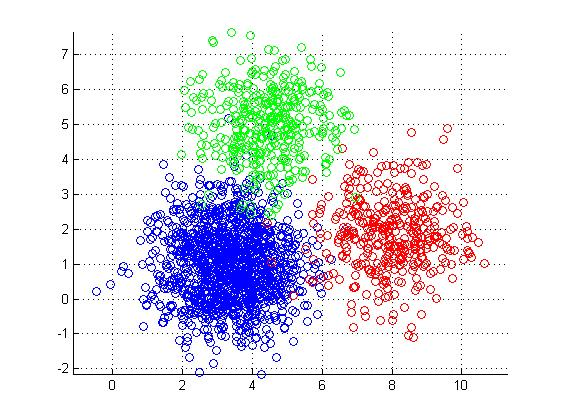
\includegraphics[width=0.8\linewidth]{sections/figures/k-means-clustering}
	\caption{Example clustering performed by the k-means-algorithm. }
	\label{fig:k-means}
\end{figure}

\subsubsection{Neural Networks}
Neural networks are at their core a purely mathematical model, however 
inspired by nature. Computational intelligence tries to mimic learning 
processes that can be found in nature. Learning is nothing more than optimizing your future decisions
based on past observations. It can be found in all kinds of mammals; and humans are the ones who excel at it. 
The structure used to learn is the brain, which consists of many
tightly knitted neurons, a special type of cell. The input and the output of each single neuron 
can be measured in voltages. 
Frank Rosenblatt (1957) developed a mathematical model to emulate the behavior of 
a single neuron. This model is called the perceptron. A single modeled
neuron consists of a set of weighted inputs, the propagation function, the activation function
and an output. Input, propagation function and activation function are set from
the beginning by the programmer or are predetermined by the data. The output
is calculated as: 
\[ f_{act.}(f_{prop.}(inputs)) \]
\[ f_{prop.}(inputs) = \sum_{i} o_{i} \cdot w_{i,j} \]

The activation function is usually picked as a gaussian or sigmoid function,
because a weighted sum of these functions is able to approximate next to every correlation.
For a single perceptron, there is only one input and one output. The result of the
propagation function comes down to a single weighted value, which is then fed
into the activation function. Comparing the output of the neural network to the 
value one would like to regress to, the weight is being adjusted. However,
this procedure reaches its limits, if there are so called hidden layers. A hidden layer
is a set of neurons which lie between the input and the output layer. Their weights
cannot be trained by simply comparing them to the desired values of the
dataset. This problem can be solved by the back propagation algorithm. Neural networks
are not limited to feed forward topologies. There is much more to explore (e.g. \cite{computational-intelligence}). 
In the context of Twitch, one could derive interests from a certain set of 
parameters. As we have just seen, neural nets have a certain accuracy, which 
is dependent on the structure and the training set fed to it. This means
that profiling users with this technology can be more revealing, the greater
the user base. 
